\subsection{What is Clustering?}
\date{}

	
	\maketitle
	
	Suppose you are working with a dataset that includes patient information from a healthcare system. The dataset is complex and includes both categorical and numeric features. You want to find patterns and similarities in the dataset. How might you approach this task?


	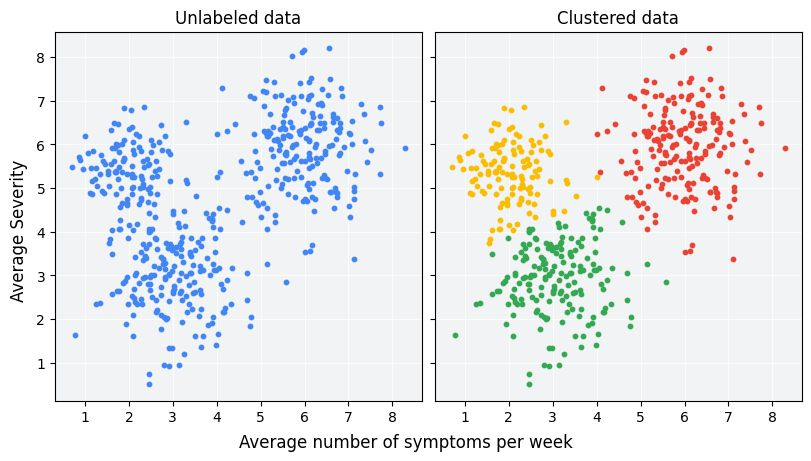
\includegraphics{one}   %picture named one in directory img
	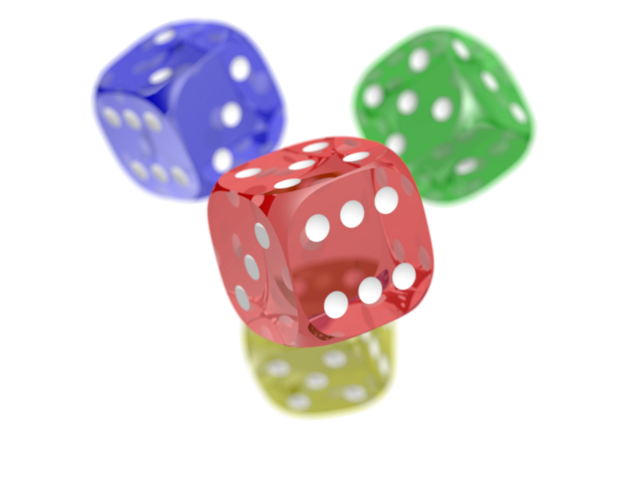
\includegraphics{dice}
	
	\par Clustering is an \textbf{unsupervised machine learning} technique designed to group unlabeled examples based on their similarity to each other. (If the examples are labeled, this kind of grouping is called \emph{classification}.) Consider a hypothetical patient study designed to evaluate a new treatment protocol. During the study, patients report how many times per week they experience symptoms and the severity of the symptoms. Researchers can use clustering analysis to group patients with similar treatment responses into clusters.The figure demonstrates one possible grouping of simulated data into three clusters.
	
\subsection{Types of clustering}

\par There are many different \textbf{clustering} algorithms as there are multiple ways to define a cluster. Different approaches will work well for different types of models depending on the size of the input data, the dimensionality of the data, the rigidity of the categories and the number of clusters within the dataset.
\subsubsection{Centroid-based clustering}

\par \textbf{Centroid-based clustering } is a method that divides a data set into similar groups based on the distance between their centroids. The \textbf{k-means} clustering algorithm is a commonly used technique, where each data point is assigned to a separate cluster. It assumes that the center of each cluster defines the cluster using a distance measure, typically Euclidean distance. The algorithm initializes the clustering by providing a number of expected clusters, which represents the 'K' in K-means. The optimal k clusters are identified by iteratively minimizing the total distance between each point and its assigned cluster centroid. \textbf{K-means} is a hard clustering approach, working well when clusters are of roughly equivalent size and there are no significant outliers or changes in density across the data. Another approach is K-medoids, which uses individual data points as the medoid or center of the cluster, making it less sensitive to outliers.

\subsubsection{Hierarchical-based clustering}

\par \textbf{Hierarchical clustering}, also known as \textbf{connectivity-based clustering}, groups data points based on their proximity and connectivity across all dimensions. It creates a \textbf{hierarchical graph network} of clusters at each hierarchical level, with each node having one parent node but multiple child nodes. These clusters can be visualized using a \textbf{dendrogram} to organize and summarize discovered clusters.

There are two approaches to performing hierarchical cluster analysis: \textbf{agglomerative} and \textbf{divisive}. \textbf{Agglomerative clustering} starts with individual data points and merges clusters by computing the \textbf{proximity matrix} of all clusters at the current level of the hierarchy. The algorithm moves to the set of newly created clusters and repeats the process until there is one \textbf{root node} at the top of the hierarchical graph.

\textbf{Divisive hierarchical clustering} methods partition data points into a \textbf{tree-like structure} using a \textbf{top-down approach}. The first step is to split the dataset into clusters using a \textbf{flat-clustering method} like \textbf{K-Means}. The clusters with the largest \textbf{Sum of Squared Errors (SSE)} are then partitioned further using a flat clustering method. The algorithm stops when it reaches individual nodes or some \textbf{minimum SSE}.

\textbf{Divisive hierarchical clustering} allows greater flexibility in terms of the \textbf{hierarchical structure} and the level of balance in different clusters. It can be faster than \textbf{agglomerative hierarchical clustering}, especially when the data doesn't require constructing the tree all the way down to individual data points.

\subsubsection{Distribution-based Clustering}

\textbf{Distribution-based clustering}, also known as \textbf{probabilistic clustering}, is a \textbf{model-based approach} that groups data points based on their \textbf{probability distribution}. This approach assumes a process generating \textbf{normal distributions} for each dimension of the data, creating \textbf{cluster centers}. It differs from \textbf{centroid-based clustering} in that it doesn't use a \textbf{distance metric} like \textbf{Euclidean} or \textbf{Manhattan distance}. Instead, it looks for a well-defined \textbf{distribution} that appears across each dimension. The \textbf{cluster means} are the means of the \textbf{Gaussian distribution} across each dimension.

One commonly used approach is the \textbf{Gaussian Mixture Model (GMM)} through \textbf{Expectation-Maximization}. This model assumes that each cluster is defined by a \textbf{Gaussian Distribution}, often called a \textbf{normal distribution}. For example, a dataset with two distinct clusters, A and B, defined by two different normal distributions, is considered. The GMM uses \textbf{Expectation-Maximization}, which starts with a random guess for the distributions along each axis and then improves iteratively by alternating two steps: 
 \\\textbf{Expectation}: assigning each data point to each cluster and computing the probability that it came from \textbf{Cluster A} and \textbf{Cluster B}; 
 \\\textbf{Maximization}: updating the parameters that define each cluster, a \textbf{weighted mean location}, and a \textbf{variance-covariance matrix} based on the likelihood of each data point being in the cluster.

Even a given point may be \textbf{probabilistically associated} with multiple clusters, making it suitable for scenarios like \textbf{diverse language preferences}.

\subsubsection{Density-based clustering}
\textbf{DBSCAN} is a \textbf{clustering algorithm} that uses \textbf{density-based clustering} to detect clusters of any shape, size, or density in data. This approach is particularly useful when working with datasets with \textbf{noise} or \textbf{outliers} or when there is no prior knowledge about the \textbf{number of clusters} in the data. DBSCAN uses a \textbf{density-based spatial clustering} approach to create clusters with a \textbf{density} passed in by the user, centered around a \textbf{spatial centroid}. The area immediately around the centroid is referred to as a \textbf{neighborhood}, and DBSCAN attempts to define neighborhoods of clusters with the specified density. For each cluster, DBSCAN defines three types of data points: \textbf{core points}, \textbf{border points}, and \textbf{outliers}.

A variant of DBSCAN, \textbf{HDBSCAN}, does not require any \textbf{parameters} to be set, making it even more flexible. HDBSCAN is less sensitive to \textbf{noise} and \textbf{outliers} in the data and can handle clusters of \textbf{varying density} more effectively. This is a primary motivation for HDBSCAN, which handles clusters of varying density more effectively than DBSCAN.

\subsection{DBSCAN}

\par As mentioned earlier, DBSCAN is a density based clustering algorithm that divides your entire dataset into dense regions separated by sparse regions.

\subsubsection{Advantages of DBSCAN}

\par \textbf{Robust to outliers :} It is robust to outliers as it defines clusters based on dense regions of data, and isolated points are treated as noise.

\par \textbf{No need to specify clusters : } Unlike some clustering algorithms, DBSCAN does not require the user to specify the number of clusters beforehand, making it more flexible and applicable to a variety of datasets.

\par \textbf{No need to specify clusters : }DBSCAN can identify clusters with complex shapes and is not constrained by assumptions of cluster shapes, making it suitable for data with irregular structures.

\par \textbf{Only 2 hyperparameters to tune : } DBSCAN has only two primary hyperparameters to tune: “eps” (distance threshold for defining neighborhood) and “min-samples” (minimum number of points required to form a dense region). This simplicity can make parameter tuning more straightforward.

\subsubsection{Disadvantages of DBSCAN}


\textbf{Sensitivity to hyperparameters : } The performance of DBSCAN can be sensitive to the choice of its hyperparameters, especially the distance threshold (eps) and the minimum number of points (min-samples). Suboptimal parameter selection may lead to under-segmentation or over-segmentation.

\textbf{Difficulty with varying density clusters : }DBSCAN struggles with clusters of varying densities. It may fail to connect regions with lower point density to the rest of the cluster, leading to suboptimal cluster assignments in datasets with regions of varying densities.

\textbf{Does not predict : } Unlike some clustering algorithms, DBSCAN does not predict the cluster membership of new, unseen data points. Once the model is trained, it is applied to the existing dataset without the ability to generalize to new observations outside the training set.


\subsubsection{Comparison with K-means}


